%
% File: introduction.tex
% Author: Eshwen Bhal
% Description: Introductory chapter.
%
\let\textcircled=\pgftextcircled
\chapter{Introduction}
\label{chap:intro}

% Hard to describe dark matter as an object. Do I call it a 'substance', 'thing', 'mass'? Can refer to it as 'non-luminous' if struggling for other adjectives

\initial{T}he universe, in all its vastness, structure, natural laws and chaos, is comprised of only three principal components: visible matter, the ingredients of stars, planets and life, is the only one we interact with on a regular basis; dark energy, a force or manifestation of something even more mysterious, responsible for the accelerating expansion of the universe, is almost entirely unknown; and dark matter, a substance invisible in all sense of the word, that binds galaxies together and influences large scale structure in the cosmos, is the focus of this thesis.


\section{Evidence for dark matter}
\label{sec:intro_dm_evidence}

The earliest evidence for a large, non-luminous component of the galaxy stretches back to the 1920s when Jacobus Kapteyn attempted to explain the motion of stars in the Milky Way \cite{1922ApJ....55..302K}. Since then, a wealth of independent astrophysical observations have reinforced the existence of this [mass] not just in our own, but in countless other galaxies and cosmological bodies. The Coma Cluster is a famous example: 90\,\% of its mass is thought to be [supplied] by dark matter, confirmed by its large mass-to-light ratio of 400 $M_{\odot} / L_{\odot}$ \cite{Yozin:2015mla}. [Other evidence] is that the rotation curves of most galaxies are roughly flat \cite{1996MNRAS-281-27P}, contrary to the expected Keplerian curve ($v \propto 1/\sqrt{r}$) expected from solely visible matter. On a galactic scale, dark matter is sprinkled in a mostly spherical halo that spans beyond the observable disc. The inclusive dark matter mass increases linearly \cite{2009arXiv0901.0632E} to compensate for the decline expressed by visible matter \cite{1970ApJ-160-811F,1992AandA-256-19B}. Gravitational lensing is another observational tool subject to be influenced by dark matter. Images of galaxies and other objects captured by this method appear distorted from a large gravitational field between the source and observer warping its local spacetime \cite{2010GReGr..42.2177H}. Arcs, ellipses and Einstein rings of smeared galaxies are often seen when dark matter is present.

While there are no widely-accepted estimations, it is believed that 85$-$95\,\% of the Milky Way's is comprised of dark matter \cite{2005MNRAS.364..433B,2006MNRAS.370.1055B,Kafle:2014xfa}. [Though] these [estimations] include non-visible identifiable matter such as dim stars, black holes and neutron stars, the term ``dark matter" typically reserved for the non-luminous, \emph{non-baryonic} matter that pervades the cosmos. From the latest results of the Planck mission, the energy density of the observable universe is composed of 26.5\,\% dark matter \cite{Aghanim:2018eyx}. This result follows the Lambda cold dark matter ($\mathrm{\Lambda}\text{CDM}$) model to describe the constituents and evolution of the universe, which is often referred to as the cosmological analog of the \acrlong{sm} of particle physics (\acrshort{sm}). From the calculations, postulations, and observations presented above, the following properties of dark matter can be deduced:

\begin{easylist}[itemize]
\ListProperties(Style*=-- , FinalMark={)}) % FinalMark indicates the end of the list properties and must always be used
& It is electrically neutral since it does not interact with electromagnetic radiation.
& It is cold (non-relativistic). Its velocity within galaxies is similar to the inhabiting stars \cite{Herzog-Arbeitman:2017fte,Bhattacharjee:2012xm}, since the combination of visible and dark matter drives the measured rotation curves. One small caveat is that galactic dark matter would be cold since a velocity above the gravitational escape velocity of the galaxy would eject high speed particles.
& It is stable, at least on the timescale of the current age of the universe. Dark matter production is postulated to have occurred only in the early universe via a thermal freeze out mechanism [REF theory section]. Hence, the remaining fraction has been present for a considerable time. Since most galaxies are dominated by dark matter and the gravitational influence from only the visible matter is too small to maintain itself, they could not have developed with out it. This supports the idea of ``bottom-up'' structure formation in the universe; smaller galaxies form around gravitational potential wells provided by coalescing dark matter, then merge to form larger structures \cite{doi:10.1093-mnras-183.3.341}.
& Its interaction with matter and itself is very weak, or even non-existent. The Bullet Cluster -- consisting of two colliding galaxies, is the best example of this inference. From measurements of predominantly x-ray emission and gravitational lensing, it was found that while there is substantial dark matter present, interaction with itself and the visible matter surrounding it was minimal at most \cite{BulletClusterDMevidence}. A kinematic explanation for the spherical distribution and low velocity of dark matter in galaxies can be explained by its collisionless nature. During the formation of a galaxy or stellar system, visible matter frequently collides, dissipating angular momentum and collapsing into a disc.
\end{easylist}


\subsection{Alternative theories to dark matter}
\label{subsec:intro_alternative_dm_theories}

Though little is known about dark matter itself since all evidence stems from its gravitational influence, there are alternative theories that may explain the observations presented above. However, the scientific community can exclude many of these. Mismeasurements of the amount of baryonic matter such as neutrinos, neutrons, and interstellar gas are among the simpler propositions.

The neutrino flux from stars, as well as the cosmic neutrino background \cite{weinberg2008cosmology}, are precise and well-tested [REF]. Even considering the upper limits on neutrino masses \cite{1742-6596-718-2-022013}, they cannot make a significant contribution to the dark matter content in the universe. This is even discounting their highly relativistic nature, where myriad experimental evidence suggests dark matter is cold.

One can also use the Cosmic Microwave Background to calculate the average photon and neutrino densities, and Big Bang Nucleosynthesis calculations to determine the baryonic matter density (see Ref. \cite{Fields:2019pfx} for results with the latest Planck mission data). These can be compared to other measurements, e.g., mass-to-light ratios averaged across the universe, to reveal a discrepancy \cite{cox2016universal}.

Neutrons cannot contribute to dark matter because isolated neutrons are unstable, decaying in a matter of minutes \cite{PDGbooklet2010}. Decay into charged protons and electrons, they interact strongly with light and therefore contribute to the luminous matter content.

\Gls{mond} is a hypothesis that aims to explain phenomena typically associated with dark matter instead by modifications to Newton's laws of motion. There exist many theories and interpretations derived from this principle, though any one strand that tries to explain an observation usually fails to satisfy other phenomena or apply to length scales that general relativity may predict well. For example, observations of the Bullet Cluster \cite{BulletClusterDMevidence} have discredited many popular \acrshort{mond} models.


\section{Overview of dark matter searches}
\label{sec:intro_dm_searches}

While observational evidence has so far lain with astrophysics, a theoretical description and discovery of dark matter may fall into the realm of particle physics with the numerous, novel experimental searches underway.  The detection of dark matter can be classified into three distinct methods with unique signatures (with a visual summary in Fig. \ref{fig:dm_detection_methods}):

\begin{easylist}[itemize]
\ListProperties(Style*=-- , FinalMark={)})
& Direct: dark matter may interact with visible matter on small scales, scattering \acrshort{sm} particles \cite{Schumann:2019eaa}. The recoil these \acrshort{sm} particles experience could be detected by highly-sensitive, low background experiments such as \acrfull{lz} \cite{kerib:2019fml} that specialises in the search for \acrshort{wimp} dark matter at a large range of masses.
& Indirect: if dark matter interacts with itself, it may annihilate to produce showers of high energy photons or pions. Background estimation is difficult since the signatures can be highly model-dependent. The photons may be of a continuum -- from hadronisation and radiation of the decay products -- or contain features, such as internal radiation from the propagator in the interaction or from loop-level processes \cite{Conrad:2017pms}. Large ranges of the annihilation cross section and dark matter mass can be probed with telescopes already searching for these [signatures].
& Production: dark matter may have been abundantly produced in the hot, early universe. High energy particle accelerators such as the \acrshort{lhc} can reproduce these conditions, with the \acrshort{wimp} miracle (see Sec. \ref{sec:dark_matter}) reinforcing the [fact dark matter may exist in these accessible mass ranges]. Many \acrfull{bsm} theories accommodate dark matter candidates with a diverse spectrum of final states that can be investigated by analysing \acrshort{lhc} data.
\end{easylist}

\begin{figure}[htbp]
    \centering
    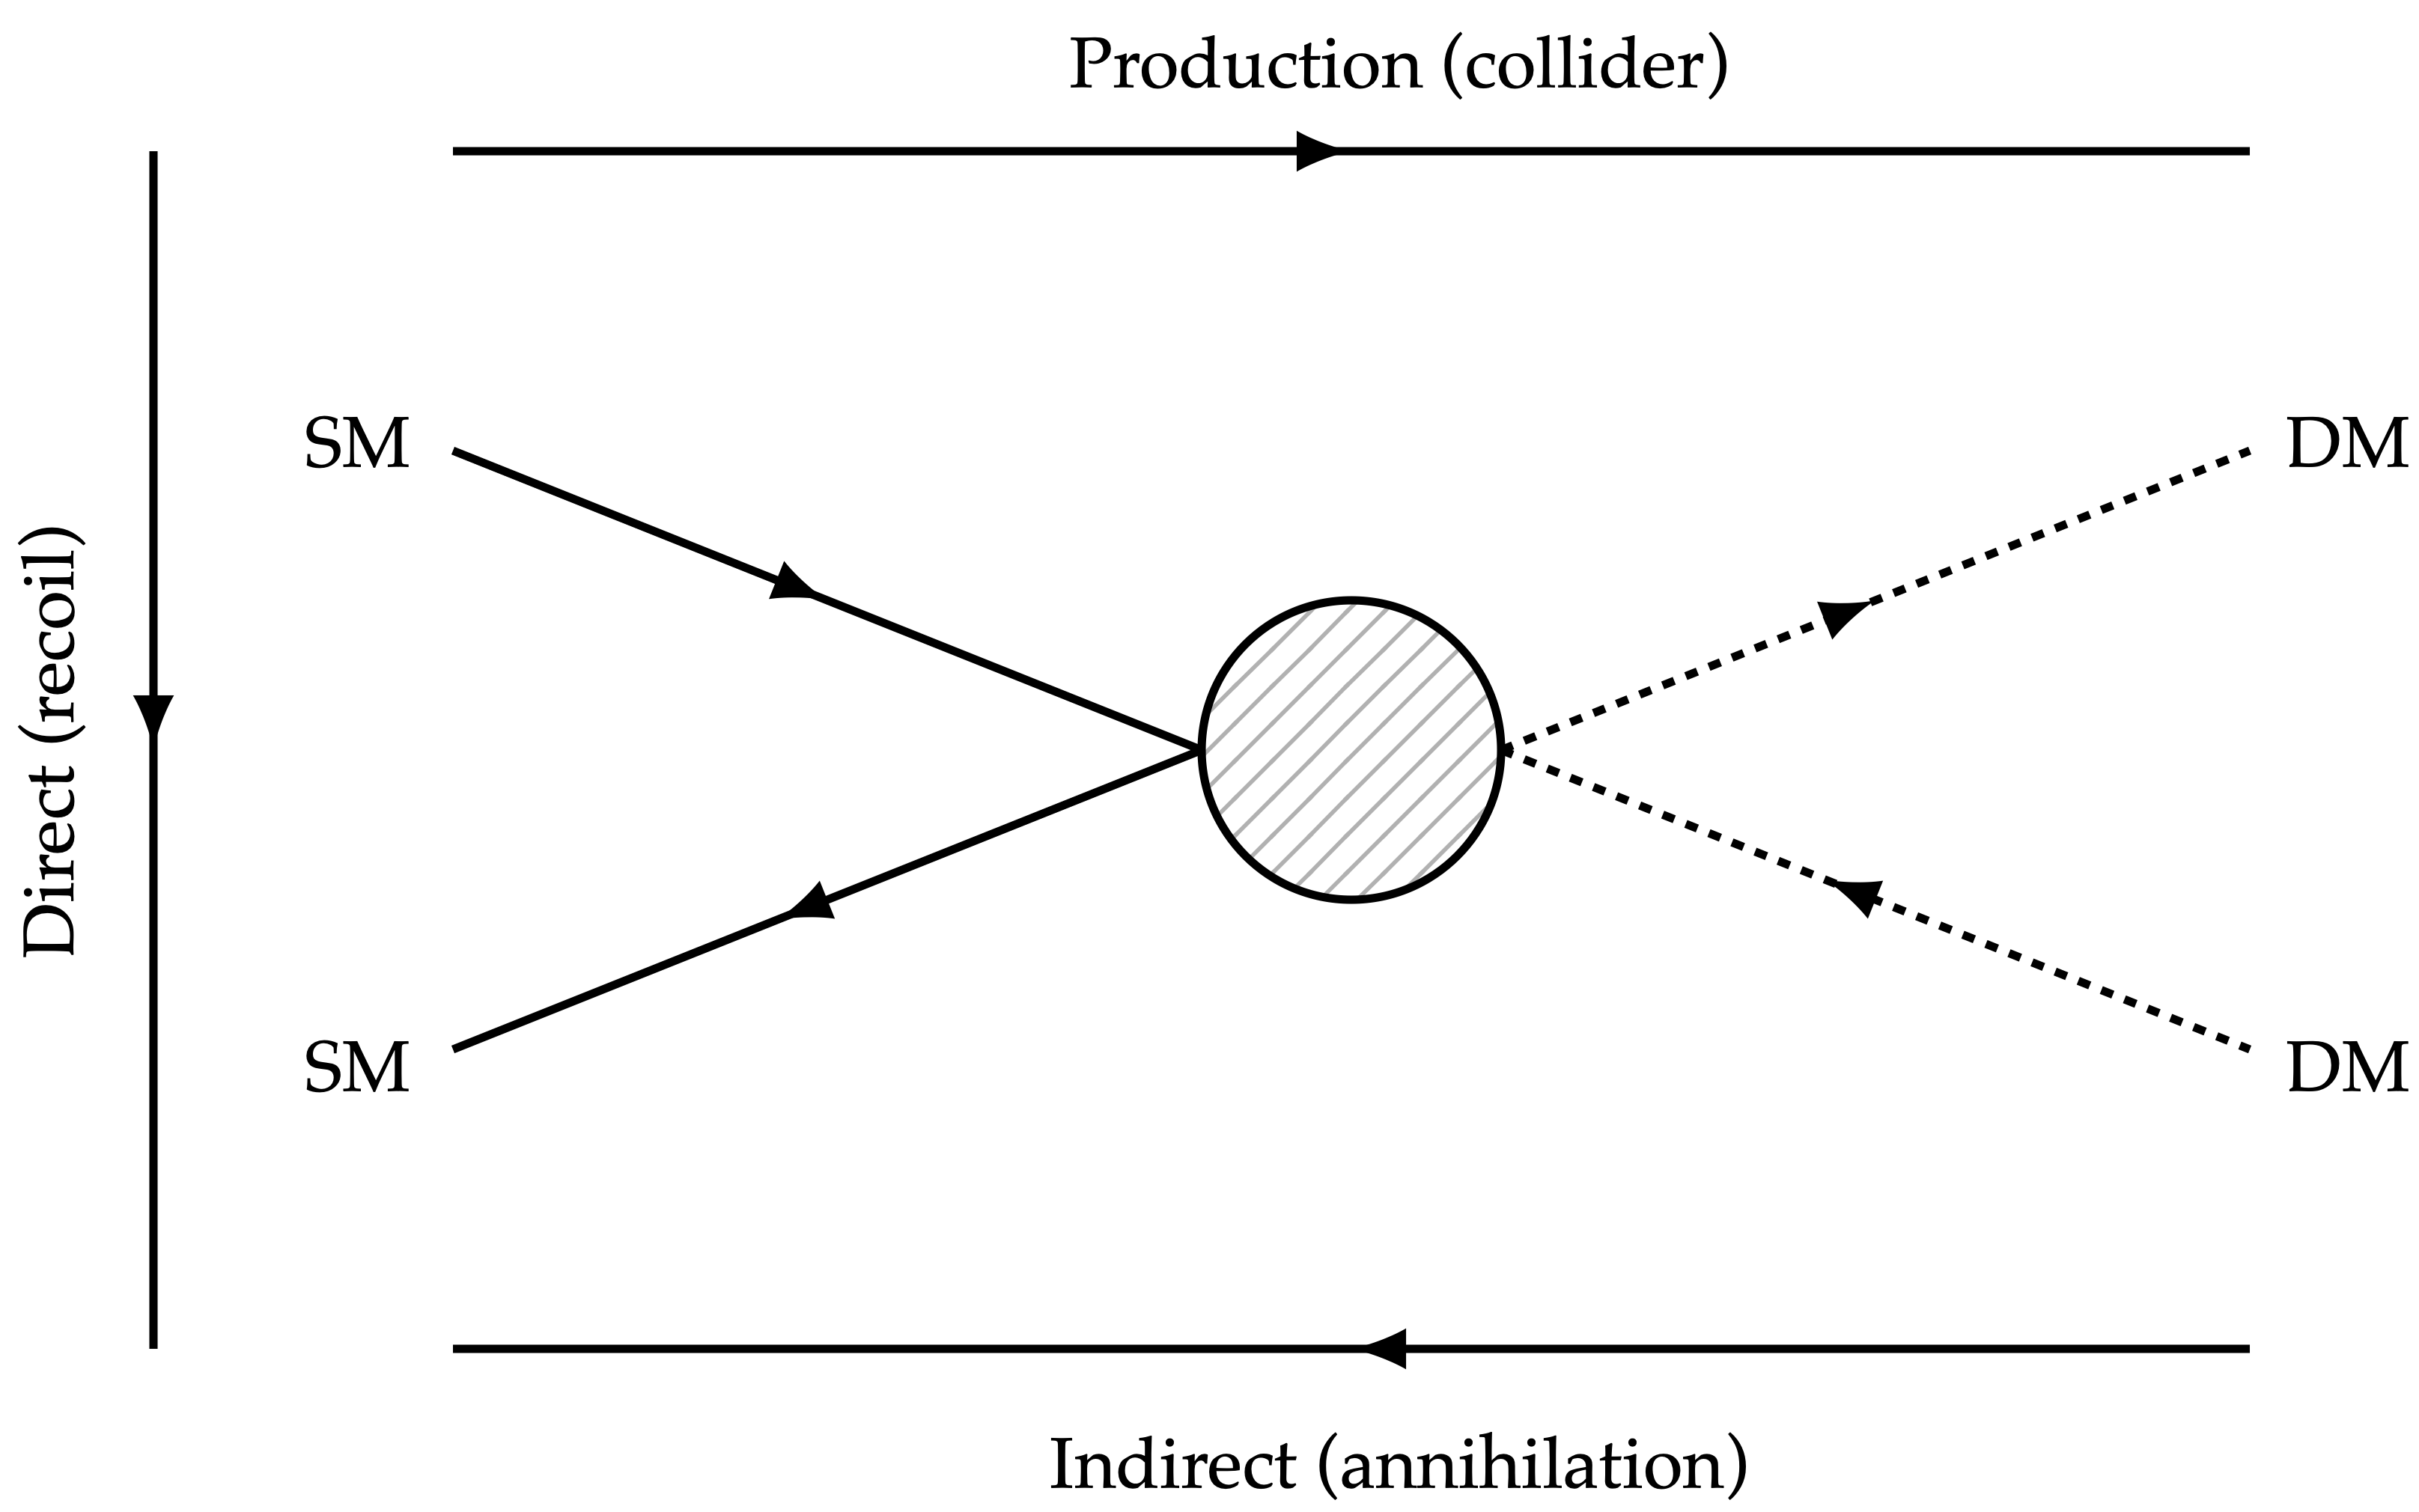
\includegraphics[width=0.75\textwidth]{figures/DM_detection_methods.png}
    \caption[A visual representation of the three main types of dark matter detection: direct, indirect, and production]{A visual representation of the three main types of dark matter detection: direct (dark matter recoiling from \acrlong{sm} particles); indirect (annihilation of dark matter); and production (dark matter created in high energy physics collisions).}
    \label{fig:dm_detection_methods}
\end{figure}


\subsection{Dark matter searches at the LHC}
\label{subsec:dm_searches_lhc}

\begin{figure}[htbp]
    \centering
    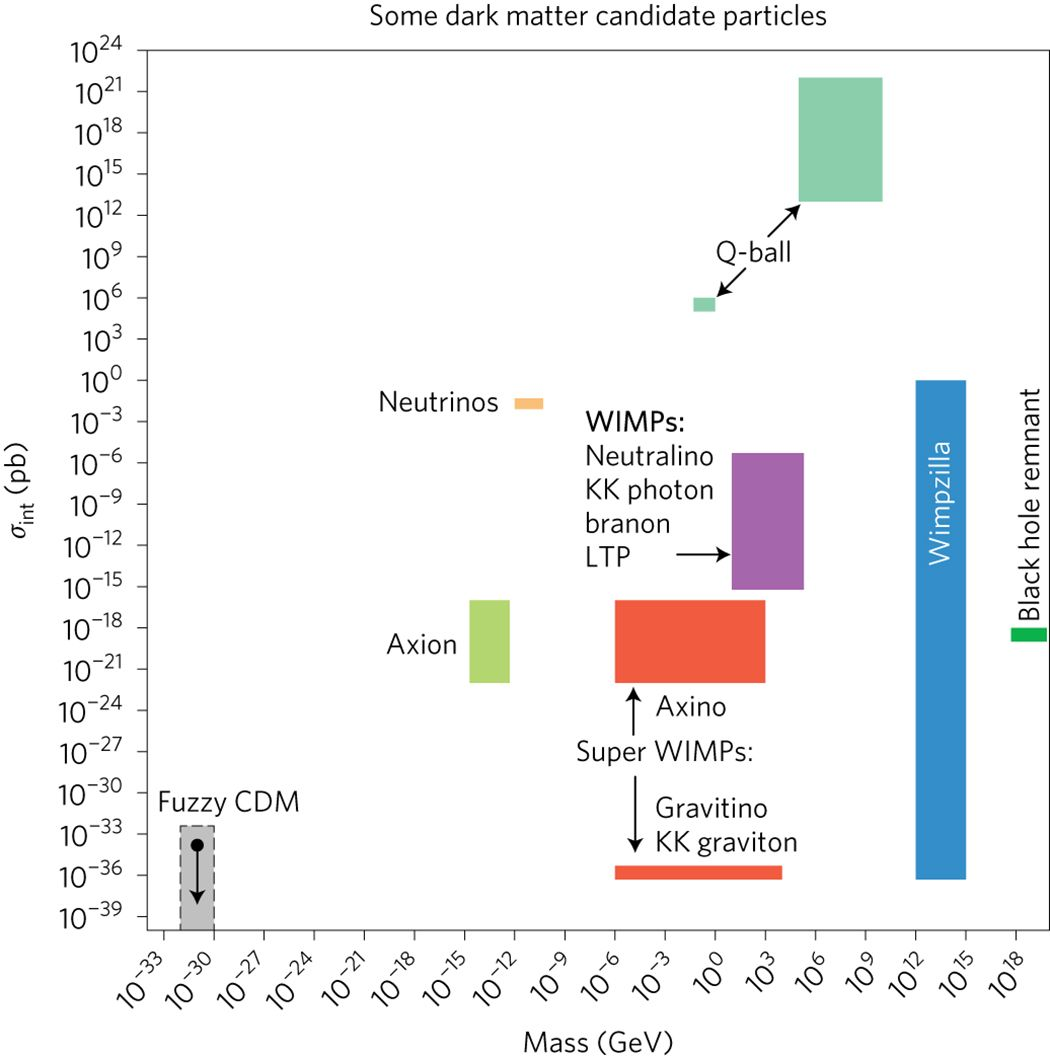
\includegraphics[width=0.6\textwidth]{figures/dm_masses_xsecs.jpg}
    \caption[The expected masses and interaction cross sections of some dark matter candidate particles. The centre of mass energy of the LHC is best suited to targeting \glspl{wimp}]{The expected masses and interaction cross sections of some dark matter candidate particles. The centre of mass energy of the LHC is best suited to targeting \glspl{wimp}. Figure taken from \cite{Conrad:2017pms}.}
\end{figure}

\iffalse

% Taken directly from second year report. Tidy up and improve. Probably only need to give an overview of things in the introduction, and save the nitty-gritty for the theory section (i.e., only mention things like WIMPs etc.). Talk about the different mechanisms for dark matter detection (direct, indirect, production), briefly touching on experiments that are looking for the former two before segueing onto production and the LHC/CMS. Briefly touch on the state of dark matter searches at the LHC and CMS (see if there are some good summary papers for ATLAS and CMS, and mention the popular theories that have dark matter candidates), then end with the fact that the foci of this thesis are hadronic searches for invisibly decaying Higgs bosons and semi-visible jets (reference chapters) with the full Run-2 dataset from CMS (will probably need to briefly describe what missing transverse energy/momentum is with their symbols).

 of dark matter searches, its production from high-energy collisions is being probed at the \acrshort{lhc}. Protons are collided at energies sufficient to produce the heavy particles that existed in the high-temperature early universe. The \acrfull{cms} experiment utilises its general purpose detector to allow physicists to search for dark matter in different theoretical frameworks.

Despite the \acrlong{sm} providing precise predictions of three of the four fundamental forces and the particles that they interact with, it does not substantiate the existence of dark matter. Several theories that are beyond (\acrshort{bsm}), or extend, the \acrlong{sm} can accommodate dark matter candidates such as sterile neutrinos \cite{doi:10.1142/S0218301313300191}, axions \cite{1981PhLB..104..199D}, and Kaluza-Klein states \cite{Han:1998sg}.

I have so far searched for dark matter in the context of \acrfull{susy} \cite{Martin:1997ns}. The theory introduces a spin symmetry that predicts a fermionic superpartner for each boson, and vice versa. If the \acrfull{lsp} is stable and electrically neutral, it would provide a promising dark matter candidate. Expected \acrshort{susy} particle decays produce the \acrshort{lsp} and, typically, hadronic jets because of the initial state particles. As \glspl{lsp} are undetectable, a reconstructed event from a detector would show a momentum imbalance. It contains ``missing" transverse energy (\glssymbol{met}) which is required to satisfy energy and momentum conservation. So the characteristics of \acrshort{susy} in a collider would be high \etmiss from the \glspl{lsp}, and several jets. But as no hint of supersymmetry has been found, other theories and simplified models from more complete theories have been considered. These are discussed later on.

There is significant motivation to study dark matter from a wider, as well as a more personal, viewpoint. It is important to understand how the universe operates, and dark matter opens up the potential for new physics that improves our understanding of nature. My personal interests include the blend of particle physics and astrophysics, and the opportunity to discover and add to humanity's collective wisdom. With a projected 130 \fbinv from the \acrshort{lhc} Run-2 at a centre-of-mass energy \comruntwo, there is great potential to constrain some of the properties of dark matter.

\fi

\newpage

\begin{easylist}[itemize]
\ListProperties(Style*=-- , FinalMark={)}, Margin=0.5cm)
& Discuss dark matter: motivation, evidence for its existence (and why it can't be neutrinos/dead stars/interstellar debris, etc.), detection methods and how we can probe it at the LHC (production).
& Briefly outline particle accelerators and their function, the fact that we can use them to potentially discover dark matter or infer more of its properties, and the models that will be discussed in more detail to try and achieve this outcome.
& The introduction probably doesn't need to be too long, maybe only a few pages. Compare length with other people's theses (ask Ben Krikler for a copy of his, look at Alex's and Lana's).
\end{easylist}

%=========================================================
